\subsection{2 Arten von Wellenausbreitung}
\begin{itemize}
	\item Transversalwellen (Transversal Polarisiert) \\
	Schwingungsrichtung $ \perp $ Ausbreitungsrichtung\\
	z.B. Seilwelle:
	\begin{center}
		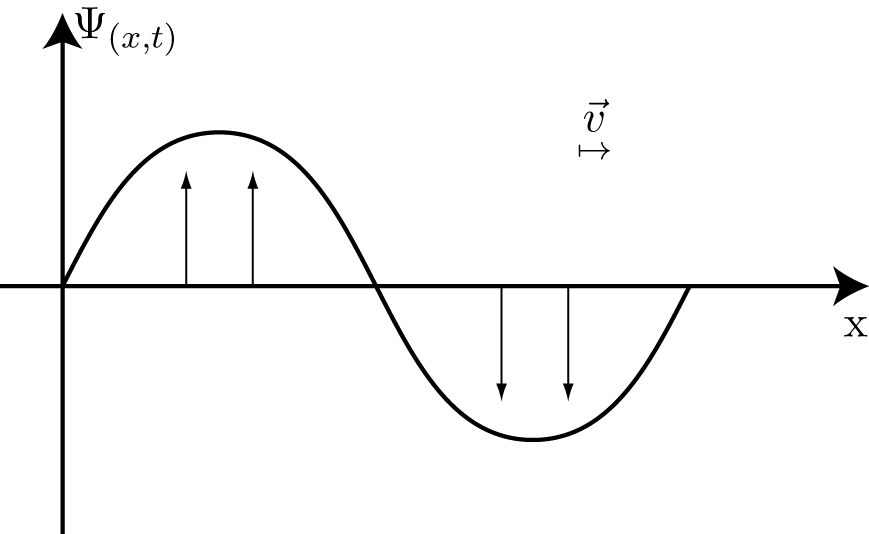
\includegraphics[width=0.5\linewidth]{skizzen/19/19B04}
	\end{center}
	\begin{center}
		
		2 Möglichkeitden der Polarisierung:
		\begin{center}
			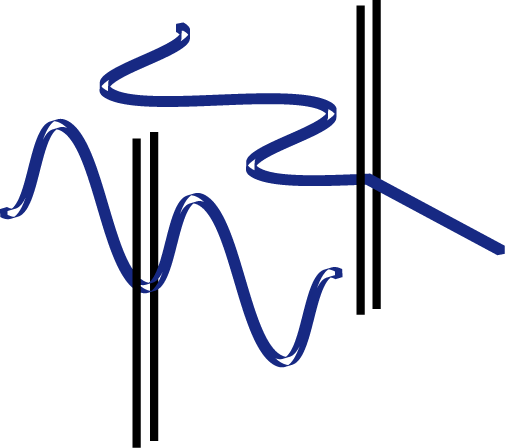
\includegraphics[width=0.5\linewidth]{skizzen/19/19B05}
		\end{center}
		Transversalwellen sind polarisierbar
	\end{center}
	\item Longitudinalwellen (longitudinal Polarisiert)\\
	z.B. Schallwellen
	\begin{center}
		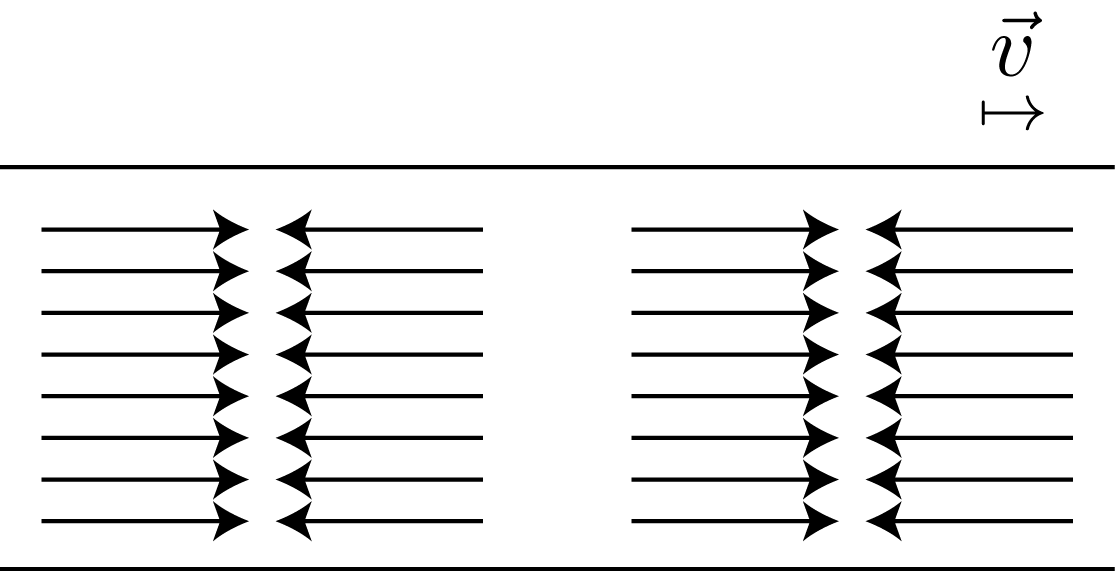
\includegraphics[width=0.5\linewidth]{skizzen/19/19B06}
	\end{center}
\end{itemize}

\underline{Mathematische Beschreibung der Wellenausbreitung}\break \\
"Störung" wandert mit Ausbreitungsgeschwindigkeit $ v_{Ph} $
\begin{center}
	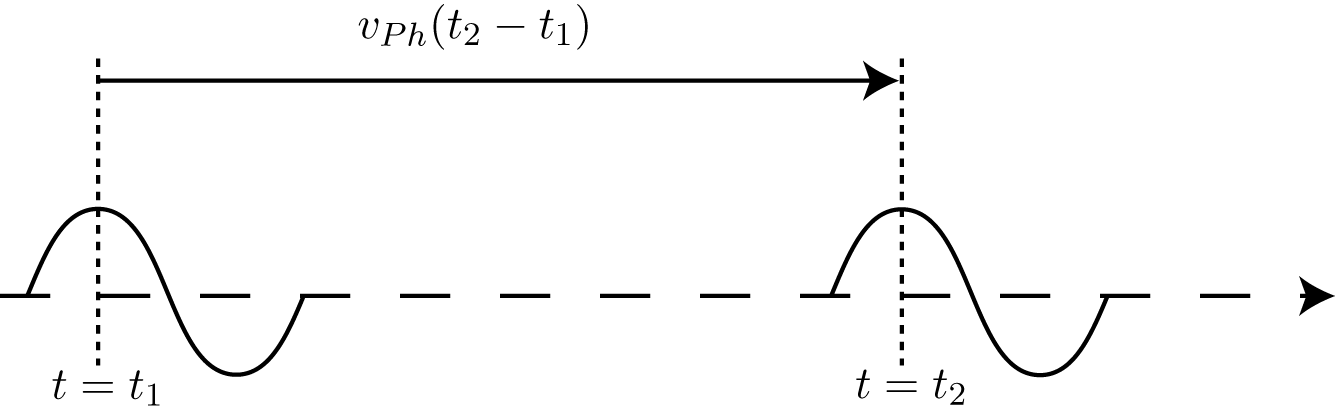
\includegraphics[width=0.7\linewidth]{skizzen/19/19B07}
\end{center}
\begin{center}
	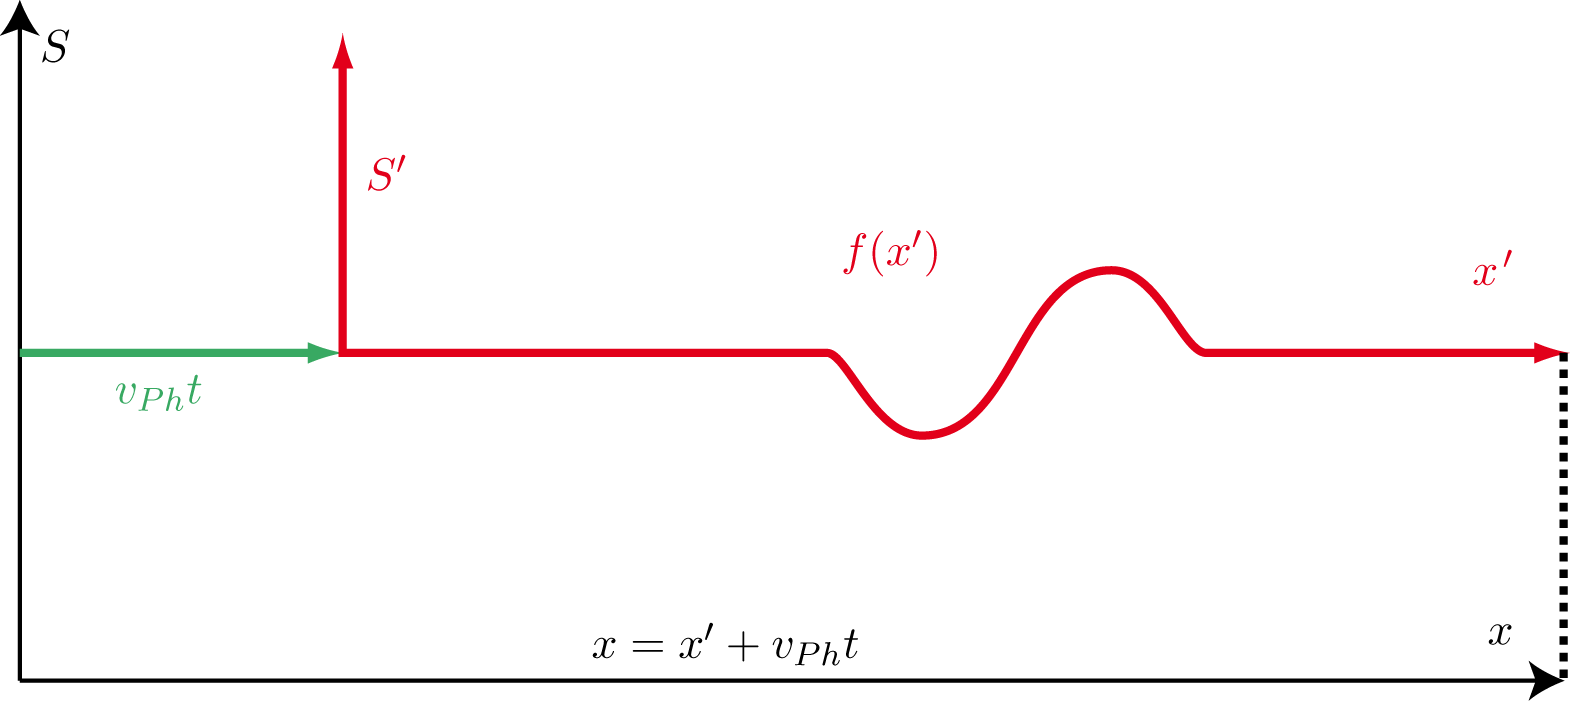
\includegraphics[width=0.7\linewidth]{skizzen/19/19B08}
\end{center}
Für mit-bewegten Beobachter bleibt Störung ortsfest (in \emph{S'})
$$ f(x')=f(x-v_{Ph}\cdot t) $$
$ \Rightarrow $ 1-dim Welle kann man beschreiben durch, $ \Psi(x,t) = \underline{\underline{f(x-v_{Ph} \cdot t)}} $ Jeder Punkt der Störung wandert mit $ v_{Ph} $ nach rechts. $$ v_{Ph} \text{: Phasengeschwindigkeit} $$
(Ausbreitung der Störung ohne Verformung!)\\
$ \Phi(x,t) $: Auslenkung, Druck, Dichte, $ \vec{E} $,$ \vec{B} $-Feld Amplitude, ...\\ \break
Sonderfall: Harmonische Wellen
\begin{align*}
\Psi(x,t) &= \Psi_0 \cdot \overbrace{\sin(K\cdot x -\omega t)}^{f(x,t)}\\
& \varphi = K \cdot x = \omega t \text{ : Phase}\\
K&: \text{Wellenzahl}\\
\omega&: \text{Kreisfrequenz}
\end{align*}
\enter\enter\enter
\hypertarget{a}{(a)} \begin{center}
	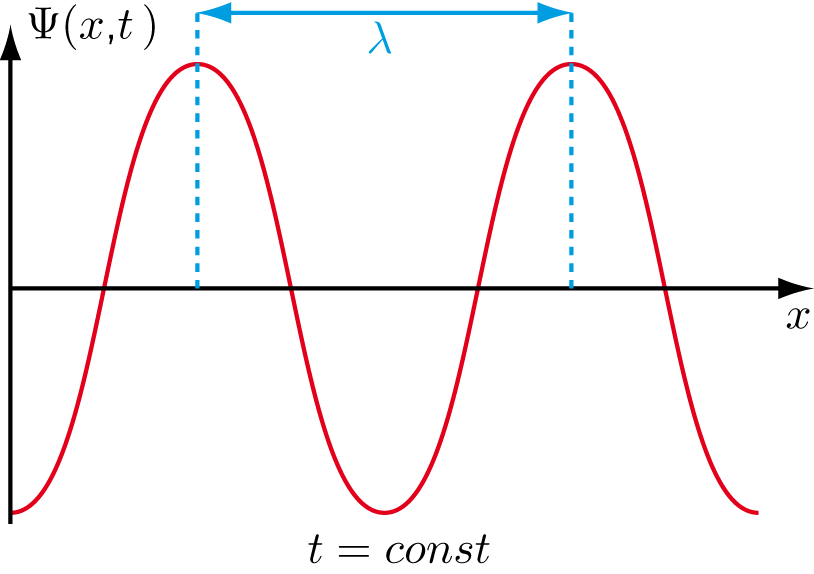
\includegraphics[width=0.5\linewidth]{skizzen/19/19B09}
\end{center}
\hypertarget{b}{(b)} \begin{center}
	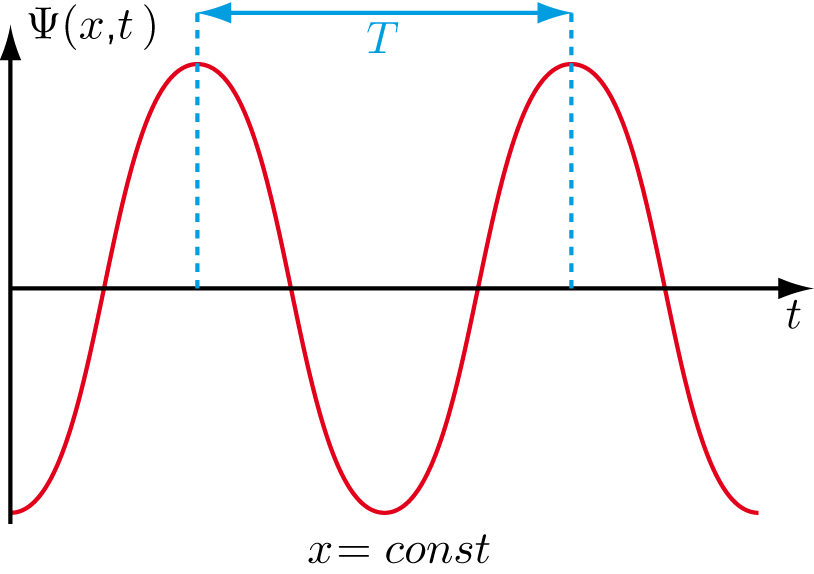
\includegraphics[width=0.5\linewidth]{skizzen/19/19B10}
\end{center}
\hyperlink{a}{(a)}
\begin{align*}
\Psi(x,t) = \Psi &= \Psi_0 \cdot \sin(Kx-\omega t)\\
&= \Psi_0 \cdot \sin(K(x+\lambda)-\omega t)\\
&= \Psi_0 \cdot \sin((Kx-\omega t)+K\cdot \lambda)\\
&\Rightarrow K \cdot \lambda = 2\pi &&\lambda \text{:Wellenlänge}\\
&\hspace{5mm} \Rightarrow K = \frac{2\pi}{\lambda}
\end{align*}
\hyperlink{b}{(b)}
\begin{align*}
\Psi &= \Psi_0 \cdot (Kx-\omega t)\\
&= \Psi_0 \cdot \sin(Kx-\omega (t+T))\\
&\Rightarrow\omega \cdot T = 2\pi \Rightarrow \omega = \frac{2\pi}{T} && \underline{T\text{: Periodendauer}}
\end{align*}

Wellen darstellbar:
\begin{align*}
\Psi(x,t) &= \Psi_0 \cdot \sin(Kx-\omega t)\\
&= \underline{\Psi_0 \cdot \sin (2\pi(\frac{x}{\lambda} - \frac{t}{T}))}
\end{align*}
In der Zeit \emph{T} (Periodendauer) breitet sich die Welle um eine Wellenlänge ($ \lambda $) aus.

$$ \Rightarrow \text{ Ausbreitungsgeschwindigketi } \boxed{ v_{Ph} = c = \frac{\lambda}{T} = \lambda \cdot \underset{\text{Frequenz}}{\nu} } $$

\begin{align*}
\Psi^{\pm}(x,t)&=\Psi_0 \cdot \sin(Kx\pm\omega t)\\
\Psi^{+} &\text{: läuft im Ortsraum nach links}\\
\Psi^{-} &\text{: läuft im Ortsraum nach rechts}
\end{align*}